\subsection{System Layer}
%\addcontentsline{toc}{subsection}{System Layer}
On the System Layer, the roles specified on the Business Layer are mapped onto a concrete data and service architecture in order to meet the requirements specified on the Functional Layer, resulting in what can be considered the technical core of the International Data Spaces.

From the requirements identified on the Functional Layer, three major technical components result:

\begin{itemize}
	\item the Connector,\par

	\item the Broker, and\par

	\item the App Store.
\end{itemize}

How these components interact with each other is depicted in Figure \ref{fig:Interaction_of_technical_components}. 


%%%%%%%%%%%%%%%%%%%% Figure/Image No: 39 starts here %%%%%%%%%%%%%%%%%%%%

\begin{figure}[H]
	\begin{Center}
		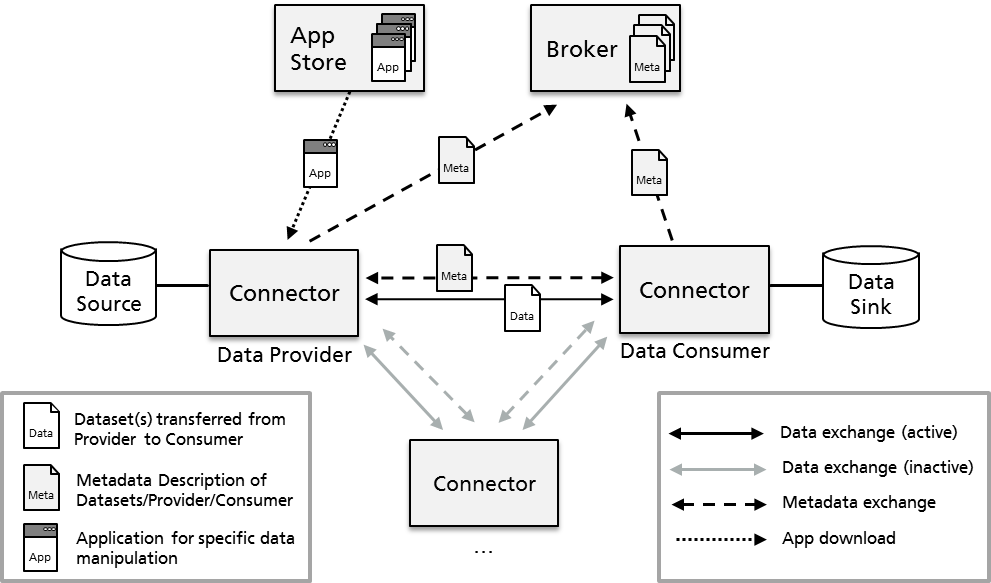
\includegraphics[width=5.31in,height=3.12in]{./media/image54.png}
		\caption{Interaction of technical components}
		\label{fig:Interaction_of_technical_components}
	\end{Center}
\end{figure}


%%%%%%%%%%%%%%%%%%%% Figure/Image No: 39 Ends here %%%%%%%%%%%%%%%%%%%%

The Connector, the Broker, and the App Store are supported by four additional components (which are not specific to the International Data Spaces, but specified for the International Data Spaces):

\begin{itemize}
	\item the Identity Provider as defined in the Security Perspective,

	\item the Vocabulary Hub currently as defined outside the IDS,
          %% ToDo: Christoph Lange: I do not understand what "outside the IDS" means here.

	\item the Update Repository (i.e. the source for updates of deployed Connectors) depending on the connectors technology, and

	\item the Trust Repository (i.e. the source for trustworthy software stacks and fingerprints as well as remote attestation checks) as discussed in the Security Perspective.
\end{itemize}

A distributed network like the International Data Spaces relies on the connection of different member nodes where Connectors or other core components are hosted (a Connector comprising one or more Data Endpoints). The Connector is responsible for the exchange of data or as a proxy in the exchange of data, as it executes the complete data exchange process (see Section 3.3.2) from and to the internal data resources and enterprise systems of the participating organizations and the International Data Spaces. It provides metadata to the Broker as specified in the connector self-description, e.g. technical interface description, authentication mechanism, exposed data sources, and associated data usage policies. It is important to note that the data is transferred between the Connectors of the Data Provider and the Data Consumer (peer-to-peer network concept).

There may be different types of implementations of the Connector, based on different technologies and depending on what specific functionality is required regarding the purpose of the Connector. Two fundamental variants are the Base Connector and the Trusted Connector (see Section 4.1) as they differ in the capabilities regarding security and data sovereignty.

Connectors can be further distinguished into External Connectors and Internal Connectors:

\begin{itemize}
	\item An External Connector executes the exchange of data between participants of the International Data Spaces. The International Data Spaces network is constituted by the total of its External Connectors. Each External Connector provides data via the Data Endpoints it exposes. Applying this principle, there is no need for a central instance for data storage. An External Connector is typically operated behind a firewall in a specially secured network segment of a participant (so-called $``$Demilitarized Zone$"$ , DMZ). From a DMZ, direct access to internal systems is not possible. It should be possible to reach an External Connector using the standard Internet Protocol (IP), and to operate it in any appropriate environment. A participant may operate multiple External Connectors (e.g., to meet load balancing or data partitioning requirements). External Connectors can be operated on-premises or in a cloud environment.

	\item An Internal Connector is typically operated in an internal company network (i.e., a network which is not accessible from outside). Implementations of Internal Connectors and External Connectors may be identical, as only the purpose and configuration differ. The main task of an Internal Connector is to facilitate access to internal data sources in order to provide data to External Connectors.
\end{itemize}

\subsubsection{Connector Architecture}
%\addcontentsline{toc}{subsubsection}{Connector Architecture}
The Connector Architecture uses application container management technology to ensure an isolated and secure environment for individual data services. A data service matches a system which offers an API to store, access or process data. To ensure privacy of sensitive data, data processing should take place as close to the data source as possible. Any data preprocessing (e.g., filtering, anonymization, or analysis) should be performed by Internal Connectors. Only data intended for being made available to other participants should be made visible through External Connectors.

Data Apps are data services encapsulating data processing and/or data transformation functionality bundled as container images for simple installation by application container management.

Using an integrated index service, the Broker manages the data sources available in the International Data Spaces and supports publication and maintenance of associated metadata. Furthermore, the Broker Index Service supports the search for data resources. Both the App Store and the Broker are based on the Connector architecture (which is described in detail in the following paragraphs) in order to support secure and trusted data exchange with these services.



%%%%%%%%%%%%%%%%%%%% Figure/Image No: 40 starts here %%%%%%%%%%%%%%%%%%%%

\begin{figure}[H]
	\begin{Center}
		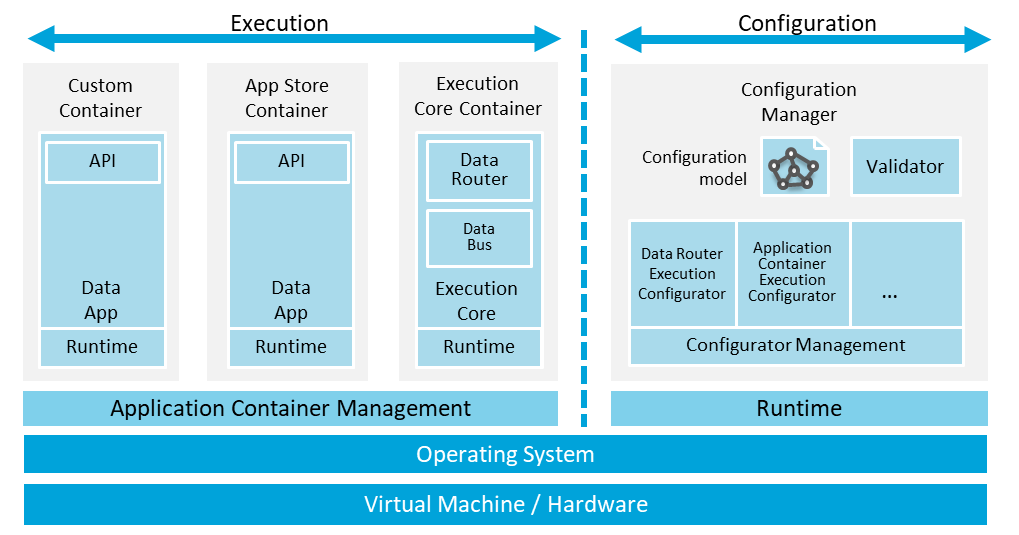
\includegraphics[width=6.37in,height=3.34in]{./media/image55.png}
		\caption{Connector Architecture}
		\label{fig:Connector_Architecture}
	\end{Center}
\end{figure}


%%%%%%%%%%%%%%%%%%%% Figure/Image No: 40 Ends here %%%%%%%%%%%%%%%%%%%%


Figure \ref{fig:Connector_Architecture} illustrates the internal structure of the Connector. A concrete installation of a Connector may differ from this structure, as existing components can be modified and optional components added. The components shown in Figure 332 can be assigned to two phases: Execution and Configuration.

The Execution phase of a Connector involves the following components:

\begin{itemize}
	\item \textit{Application Container Management}: In most cases, the deployment of an Execution Core Container and selected Data Services is based on application containers. Data Services are isolated from each other by containers in order to prevent unintended interdependencies. Using Application Container Management, extended control of Data Services and containers can be enforced. During development, and in case of systems with limited resources, Application Container Management can be omitted. Difficulties in container deployment can be handled by special Execution Configurators (see below).

	\item An \textit{Execution Core Container} provides components for interfacing with Data Services and supporting communication (e.g., Data Router or Data Bus to a Connector).

	\begin{itemize}
		\item A \textit{Data Router} handles communication with Data Services to be invoked according to predefined configuration parameters. In this respect, it is responsible of how data is sent (and received) to (and from) the Data Bus from (and to) Data Services. Participants have the option to replace the Data Router component by alternative implementations of various vendors. Differences in configuration can be handled by specialized Execution Configurator plug-ins. If a Connector in a limited or embedded platform consists of a single Data Service or a fixed connection configuration (e.g., on a sensor device), the Data Router can be replaced by a hard-coded software, or the Data Service can be exposed directly. The Data Router invokes relevant components for the enforcement of Usage Policies, e.g. a Policy Enforcement Point (see section 4.1.3.6), as configured in the connector or specified in the Usage Policy.

		\item The \textit{Data Bus} exchanges data with Data Services and Data Bus components of other Connectors. It may also store data within a Connector. Usually, the Data Bus provides the method to exchange data between Connectors. Like the Data Router, the Data Bus can be replaced by alternative implementations in order to meet the requirements of the operator. The selection of an appropriate Data Bus may depend on various aspects (e.g., costs, level of support, throughput rate, quality of documentation, or availability of accessories).

	\end{itemize}

	\item An \textit{App Store Container} is a certified container downloaded from the App Store, providing a specific Data Service to the Connector.

	\item A \textit{Custom Container} provides a self-developed Data Service. Custom containers usually require no certification.

	\item A \textit{Data Service} defines a public API, which is invoked from a Data Router. This API is formally specified in a meta-description that is imported into the configuration model. The tasks to be executed by Data Services may vary. Data Services can be implemented in any programming language and target different runtime environments. Existing components can be reused to simplify migration from other integration platforms.

	\item The \textit{Runtime} of a Data Service depends on the selected technology and programming language. The Runtime together with the Data Service constitutes the main part of a container. Different containers may use different runtimes. What runtimes are available depends only on the base operating system of the host computer. From the runtimes available, a service architect may select the one deemed most suitable.

\end{itemize}

The Configuration phase of a Connector involves the following components:

\begin{itemize}
	\item The \textit{Configuration Manager} constitutes the administrative part of a Connector. Its main task is the management and validation of the Configuration Model, followed by deployment of the Connector. Deployment is delegated to a collection of Execution Configurators by the Configurator Management.

	\item The \textit{Configuration Model} is an extendable domain model for describing the configuration of a Connector. It consists of technology-independent, inter-connected configuration aspects.

	\item \textit{Configurator Management} loads and manages an exchangeable set of Execution Configurators. When a Connector is deployed, the Configurator Management delegates each task to a special Execution Configurator.

	\item \textit{Execution Configurators} are exchangeable plug-ins which execute or translate single aspects of the Configuration Model to a specific technology. The procedure of executing a configuration depends on the technology used. Common examples would be the generation of configuration files or the usage of a configuration API. Using different Execution Configurators, it is possible to adopt new or alternative technologies and integrate them into a Connector. Therefore, every technology (operating system, application container management, etc.) gets its own Execution Configurator.

	\item The \textit{Validator} checks if the Configuration Model complies with self-defined rules and with general rules specified by the International Data Spaces, respectively. Violation of rules can be treated as warnings or errors. If such warnings or errors occur, deployment may fail or be rejected.
\end{itemize}

As the Configuration phase and the Execution phase are separated from each other, it is possible to develop, and later on operate, these components independently of each other. Different Connector implementations may use various kinds of communication and encryption technologies, depending on the requirements given.

\paragraph{Connector Configuration Model\\}
%\addcontentsline{toc}{paragraph}{Connector Configuration Model}
The Connector Configuration Model describes the configuration of a Connector, which is set-up during deployment. The model is technology-independent. A Connector can be configured for different statuses (development, test, or live). 



%%%%%%%%%%%%%%%%%%%% Figure/Image No: 41 starts here %%%%%%%%%%%%%%%%%%%%

\begin{figure}[H]
	\begin{Center}
		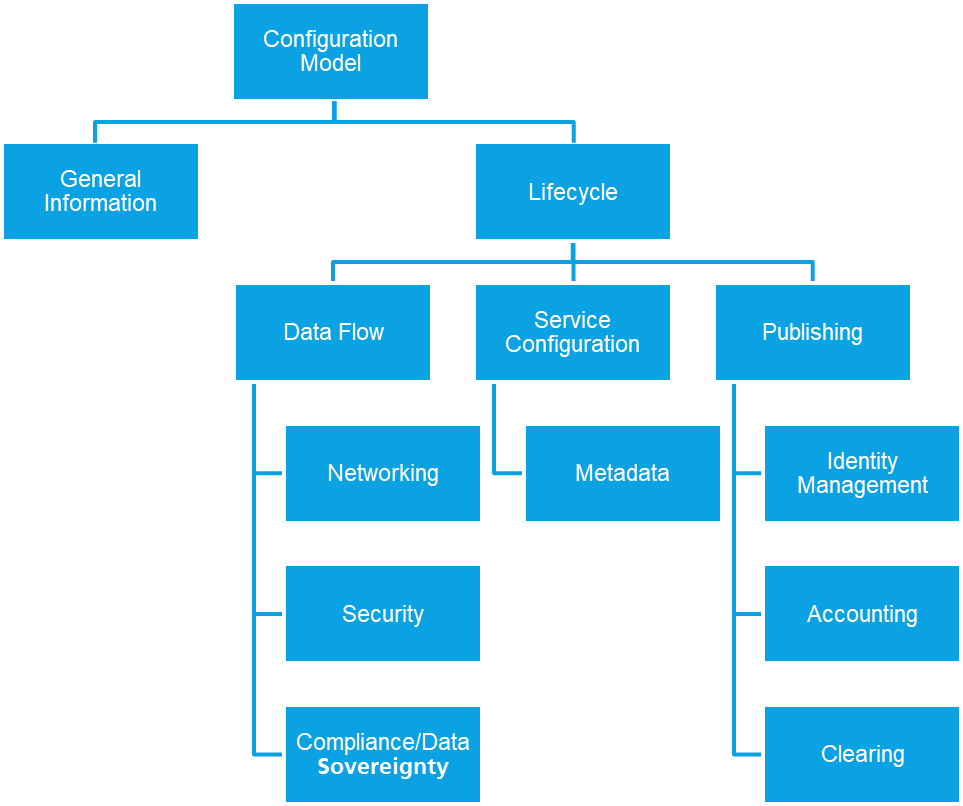
\includegraphics[width=6.42in,height=5.37in]{./media/image56.png}
		\caption{Connector Configuration Model}
		\label{fig:Connector_Configuration_Model}
	\end{Center}
\end{figure}


%%%%%%%%%%%%%%%%%%%% Figure/Image No: 41 Ends here %%%%%%%%%%%%%%%%%%%%



The components of the Connector Configuration Model are implemented with the help of special Execution Configurators:


\begin{itemize}
	\item $``$General Information$"$  includes the configuration type, the Connector type (Base, Trusted, Mobile, Embedded, Developer), the Connector version, a timestamp of the last change made to the configuration, the configuration status (development, test, live), and a name of a contact person.

	\item $``$Lifecycle$"$  contains information on the Data Flow, the Service Configuration, and Publishing.

	\begin{itemize}
		\item $``$Data Flow$"$  defines the configuration of tasks and connections established by the Data Router between the Data Services and the Data Bus (for multiple data pipelines).

		\begin{itemize}
			\item $``$Networking$"$  relates to the definition of network parameters (ports, IPs, etc.) for being used inside the Connector as well as for connections to External Connectors.

			\item $``$Security$"$  contains information about, for example, which SSL certificates should be used for connections, or which public key infrastructure should be used.

			\item $``$Compliance / Data Sovereignty$"$  specifies rules to be checked by the Validator before Connector deployment. If warnings or errors occur, deployment may be canceled. This feature is used to prevent incorrect configuration of the Connector.

		\end{itemize}

		\item $``$Service Configuration$"$  defines how configuration parameters for Data Services or other Connector components have to be set.

		\item $``$Metadata$"$  describes the data types for input and output used by different Connector components (see chapter 3.4.5 - App Interfaces). Data Services can provide metadata descriptions, which can be imported to the Configuration Model. This information is used to configure the Data Flow.

		\item $``$Publishing$"$  defines which Data Flows or Data Services are provided to external participants. This information is submitted to a Broker.

		\begin{itemize}
			\item $``$Identity Management$"$  defines the Identity Provider, which is closely integrated with the Connector. To be able to connect to an Identity Provider, a Data Service may need additional libraries.

			\item For $``$Accounting$"$  of a data exchange transaction between participants, it is necessary to record additional information, such as contract specifications, pricing models, or billing details.

			\item $``$Clearing$"$  describes which Clearing House should be informed regarding a certain data exchange transaction.
		\end{itemize}
	\end{itemize}
\end{itemize}


\paragraph{Special Connector Implementations\\}
%\addcontentsline{toc}{paragraph}{Special Connector Implementations}
What type of Connector is to be implemented may depend on various aspects, such as the execution environment given or the current developmental stage regarding Data Services or Data Flows used. In the following, three exemplary scenarios are outlined:

\subparagraph*{Developer Connector}
As is the case for the development of any software, developing Data Services or configuring Data Flows comprises several phases (specification, implementation, debugging, testing, profiling, etc.). For reasons of simplification, it may be useful to run Connectors without application container management. In doing so, the development process can be accelerated, as packing and starting the container can be omitted, and debugging can be done in the development environment. After successfully passing all tests, the configuration model used for the Developer Connector can be used to deploy a productive (live) Connector. Upon deployment in the live environment, the Connector is ready for being used.

\subparagraph*{Mobile Connector}
Mobile operating systems (e.g., Android, iOS, or Windows Mobile) use platforms with limited hardware resources. In such environments, application container management is not necessarily required. The same applies for operating systems which do not support application containers, or systems without any operating system (e.g. microcontrollers). In such environments, Data Services (and the execution core) can be started directly on the host system, without requiring any virtualization. The differences between Connectors \textit{with} containers and Connectors \textit{without} containers can be met by different Execution Configurator modules.

\subparagraph*{Embedded Connector}
Another way of Connector miniaturization offers the Embedded Connector. Embedded Connectors have the same design as Mobile Connectors, and do not necessarily require application container management either. However, unlike Mobile or Developer Connectors, the Configuration Manager is not part of the Connector hardware platform here, which is why remote configuration capabilities of the platform are required (e.g., using an API or configuration files).

Additional steps for Connector miniaturization may include the use of a common runtime for all components, or simplified versions of the Data Router and the Data Bus. If data is to be sent to a fixed recipient only, a simple Data Bus client library may be sufficient. Similarly, it may be sufficient to hard-code a single, fixed connection to the Data Bus instead of using a configurable component. To save communication overhead, simple API calls inside the common runtime could be used.

\subsubsection{Meta Data Broker}
%\addcontentsline{toc}{subsubsection}{Broker}

%old
%The IDS Broker consists of an IDS Connector (see section 3.5.1), a service for data source registration, publication, maintenance, and query, based on an index. Therefore, for any interaction with the IDS Broker the processes defined on the Process Layer, the descriptions defined on the Information Layer, and descriptions defined on the System Layer can be applied. The Information Layer describes the message types for Broker registration and query. An IDS Broker may provide additional services that must be described by the IDS Information Model. 

%new
The IDS Meta Data Broker is a service for publishing and searching metadata of connectors and resources between International Data Spaces Participants. In order to ensure the necessary interoperability and general interactions, an IDS Meta Data Broker is also defined as a specialized IDS Connector. The communication between an IDS Connector and an IDS Meta Data Broker is based on the same principles as any other Connector-Connector communication within the International Data Spaces. Still, an IDS Meta Data Broker provides a collection of additional functionalities:
\begin{itemize}
	\item Indexing services in order to effectively and efficiently respond to queries and present known Connectors and other resources
	\item Interfaces for Users or IDS-Messages to ensure access to the stored information. 
\end{itemize}


The capabilities and functionalities of an IDS Meta Data Broker are subject of IDS Certification. After a successful certification of the relevant Criteria of an IDS Connector and as an IDS Meta Data Broker, a software component can include the following RDF statement into its Self-Description:
 
\begin{verbatim}
<Connector/Broker URI>
<http://www.w3.org/1999/02/22-rdf-syntax-ns#type>
<https://w3id.org/idsa/core/Broker> .
\end{verbatim}
\todo{make a listing with numbering out of this}

In accordance to the thereby directly included guaranteed features, an IDS conform Meta Data Broker may provide significantly more services. Several options to include broker features in an International Data Space are possible: 
\begin{itemize}
	\item only mandatory IDS Meta Data Broker features as specifed in the IDS Meta Data Broker Specification\footnote{ToDo Link},
	\item mandatory and optional features as specifed in the IDS Meta Data Broker Specification,
	\item general features supporting publication, indexing and discovery which are not mentioned in this as specifed in the IDS Meta Data Broker Specification (not applicable as an IDS Meta Data Broker, if they interfere with mandatory features), or
	\item any combination of the first three categories.
\end{itemize}


\subsubsection{Data Apps and App Store}
%\addcontentsline{toc}{subsubsection}{Data Apps and App Store}
As described in section 3.5.1 Connectors can make use of Apps for several purposes. Three types of Data Apps can be distinguished:

\begin{itemize}
	\item self-developed Data Apps, which are used by the Data Provider's own Connector (usually requiring no certification from the Certification Body),

	\item third-party Data Apps, which are retrieved from the App Store (and which may require certification), and

	\item Data Apps provided by the Connector of the Data Consumer, which allow the Data Provider to use certain functions before data is exchanged, e.g., filtering or aggregation of data (which may also require certification).
\end{itemize}

In addition, Data Apps can be divided into three categories:

\begin{itemize}
	\item System Adapters are Data Apps establishing interfaces to external enterprise information systems. The main tasks System Adapters is providing access to enterprise information systems and, if necessary, transforming from an internal data model to a data model applicable for data a exchange (e.g., a standard or recommendation for a given application domain), as well as to enrich the data with the required
	metadata to exchange information with other Connectors. System Adapters can be used by Data Providers and Data Consumers, i.e., for reading and writing data to enterprise information systems. 

	\item Smart Data Apps execute any kind of data processing or transformation. Normally, the data provided by, or sent to, a Smart Data App is already annotated with metadata (as described in the Information Layer section). The important difference to System Adapters is that Smart Data Apps have input \emph{and} output data, as they process the input data to provide value-added
	output data. For example, a Smart Data App could apply a data transformation (e.g., from miles into meters or from XML into JSON) or apply machine learning to do classification (e.g., to recognize malicious
	behavior of a machine).

	\item Management Apps provide additional functionality within a Connector, but do not deal directly with the data being exchanged. For example, Usage Policies can enforce the processing of the data in a trusted environment, i.e., a Trusted Connector. A monitoring app could provide statistical information about data usage to a Data Provider.
\end{itemize}



The IDS App Store is a secure platform for distributing Data Apps and features different search options (e.g., by functional or non-functional properties, pricing model, certification status, community ratings, etc.). An IDS App Store consists of a registry for available Data Apps in this App Store. Therefore, an App Store supports operations for Data App registration, publication, maintenance, and query, as well as operations for the provisioning of a Data App to a connector. These basic operations can be complemented by additional services, e.g., billing or support activities. 

\todo{Hier Verweis auf Jive-Dokument hinzufügen? : https://industrialdataspace.jiveon.com/docs/DOC-2604}
